%%% TeX代码开始

\documentclass[UTF8,9pt]{ctexbeamer}

\usetheme{Boadilla}

\usecolortheme{beaver}

\usepackage{graphicx}

\usepackage{color}
\usepackage{subfigure}

\setbeamertemplate{caption}[numbered]
\graphicspath{{Images/}}
\begin{document}

\title{{电子元件散热仿真}\\\vspace{1em}}

\subtitle{传热学课程汇报}

\author{\songti {Name}}

\institute{}

\date{\today}

\frame{\titlepage}

\begin{frame}{目录}

\tableofcontents

\end{frame}

\section{物理问题简介}

\begin{frame}{目录}

\tableofcontents[currentsection]

\end{frame}

\begin{frame}

\frametitle{物理问题描述}
%
% \vfill
电子元件安装在PCB板上,使用板状散热器,在自然对流条件下运行。
\\

\begin{figure}
    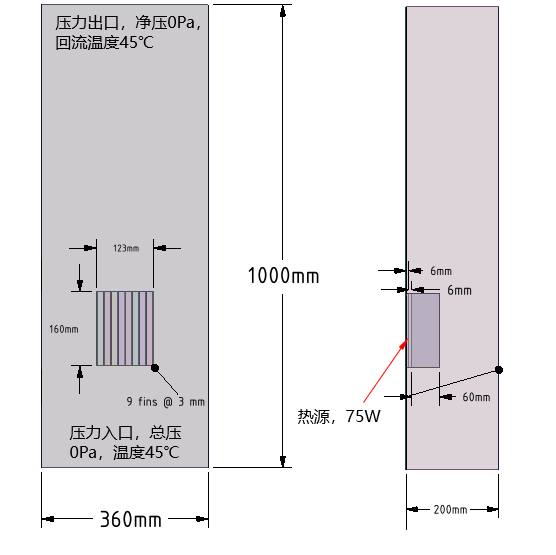
\includegraphics[height=6cm]{figure2.png}
    \caption{问题描述}
\end{figure}
%

%
\end{frame}


\section{CFD 仿真过程}

\begin{frame}

\frametitle{目录}

\tableofcontents[currentsection]

\end{frame}

\begin{frame}{模型与方法}
	\begin{table}[]
		\begin{tabular}{l|l}
		\hline
		Model           & Settings           \\ \hline
		Space           & 3D                 \\
		Time            & Steady             \\
		Viscous         & Laminar            \\ 
		Heat   Transfer & Enabled            \\
		Radiation       & Surface to Surface \\
        \hline
		\end{tabular}
		\caption[]{计算模型设置。}
	\end{table}
\end{frame}



% \end{frame}
\begin{frame}{无辐射模型}
	% \vfill
	\begin{figure}[htbp]
		\centering
		\subfigure[]
		{
		%  \begin{minipage}{5cm}
		  \centering
		  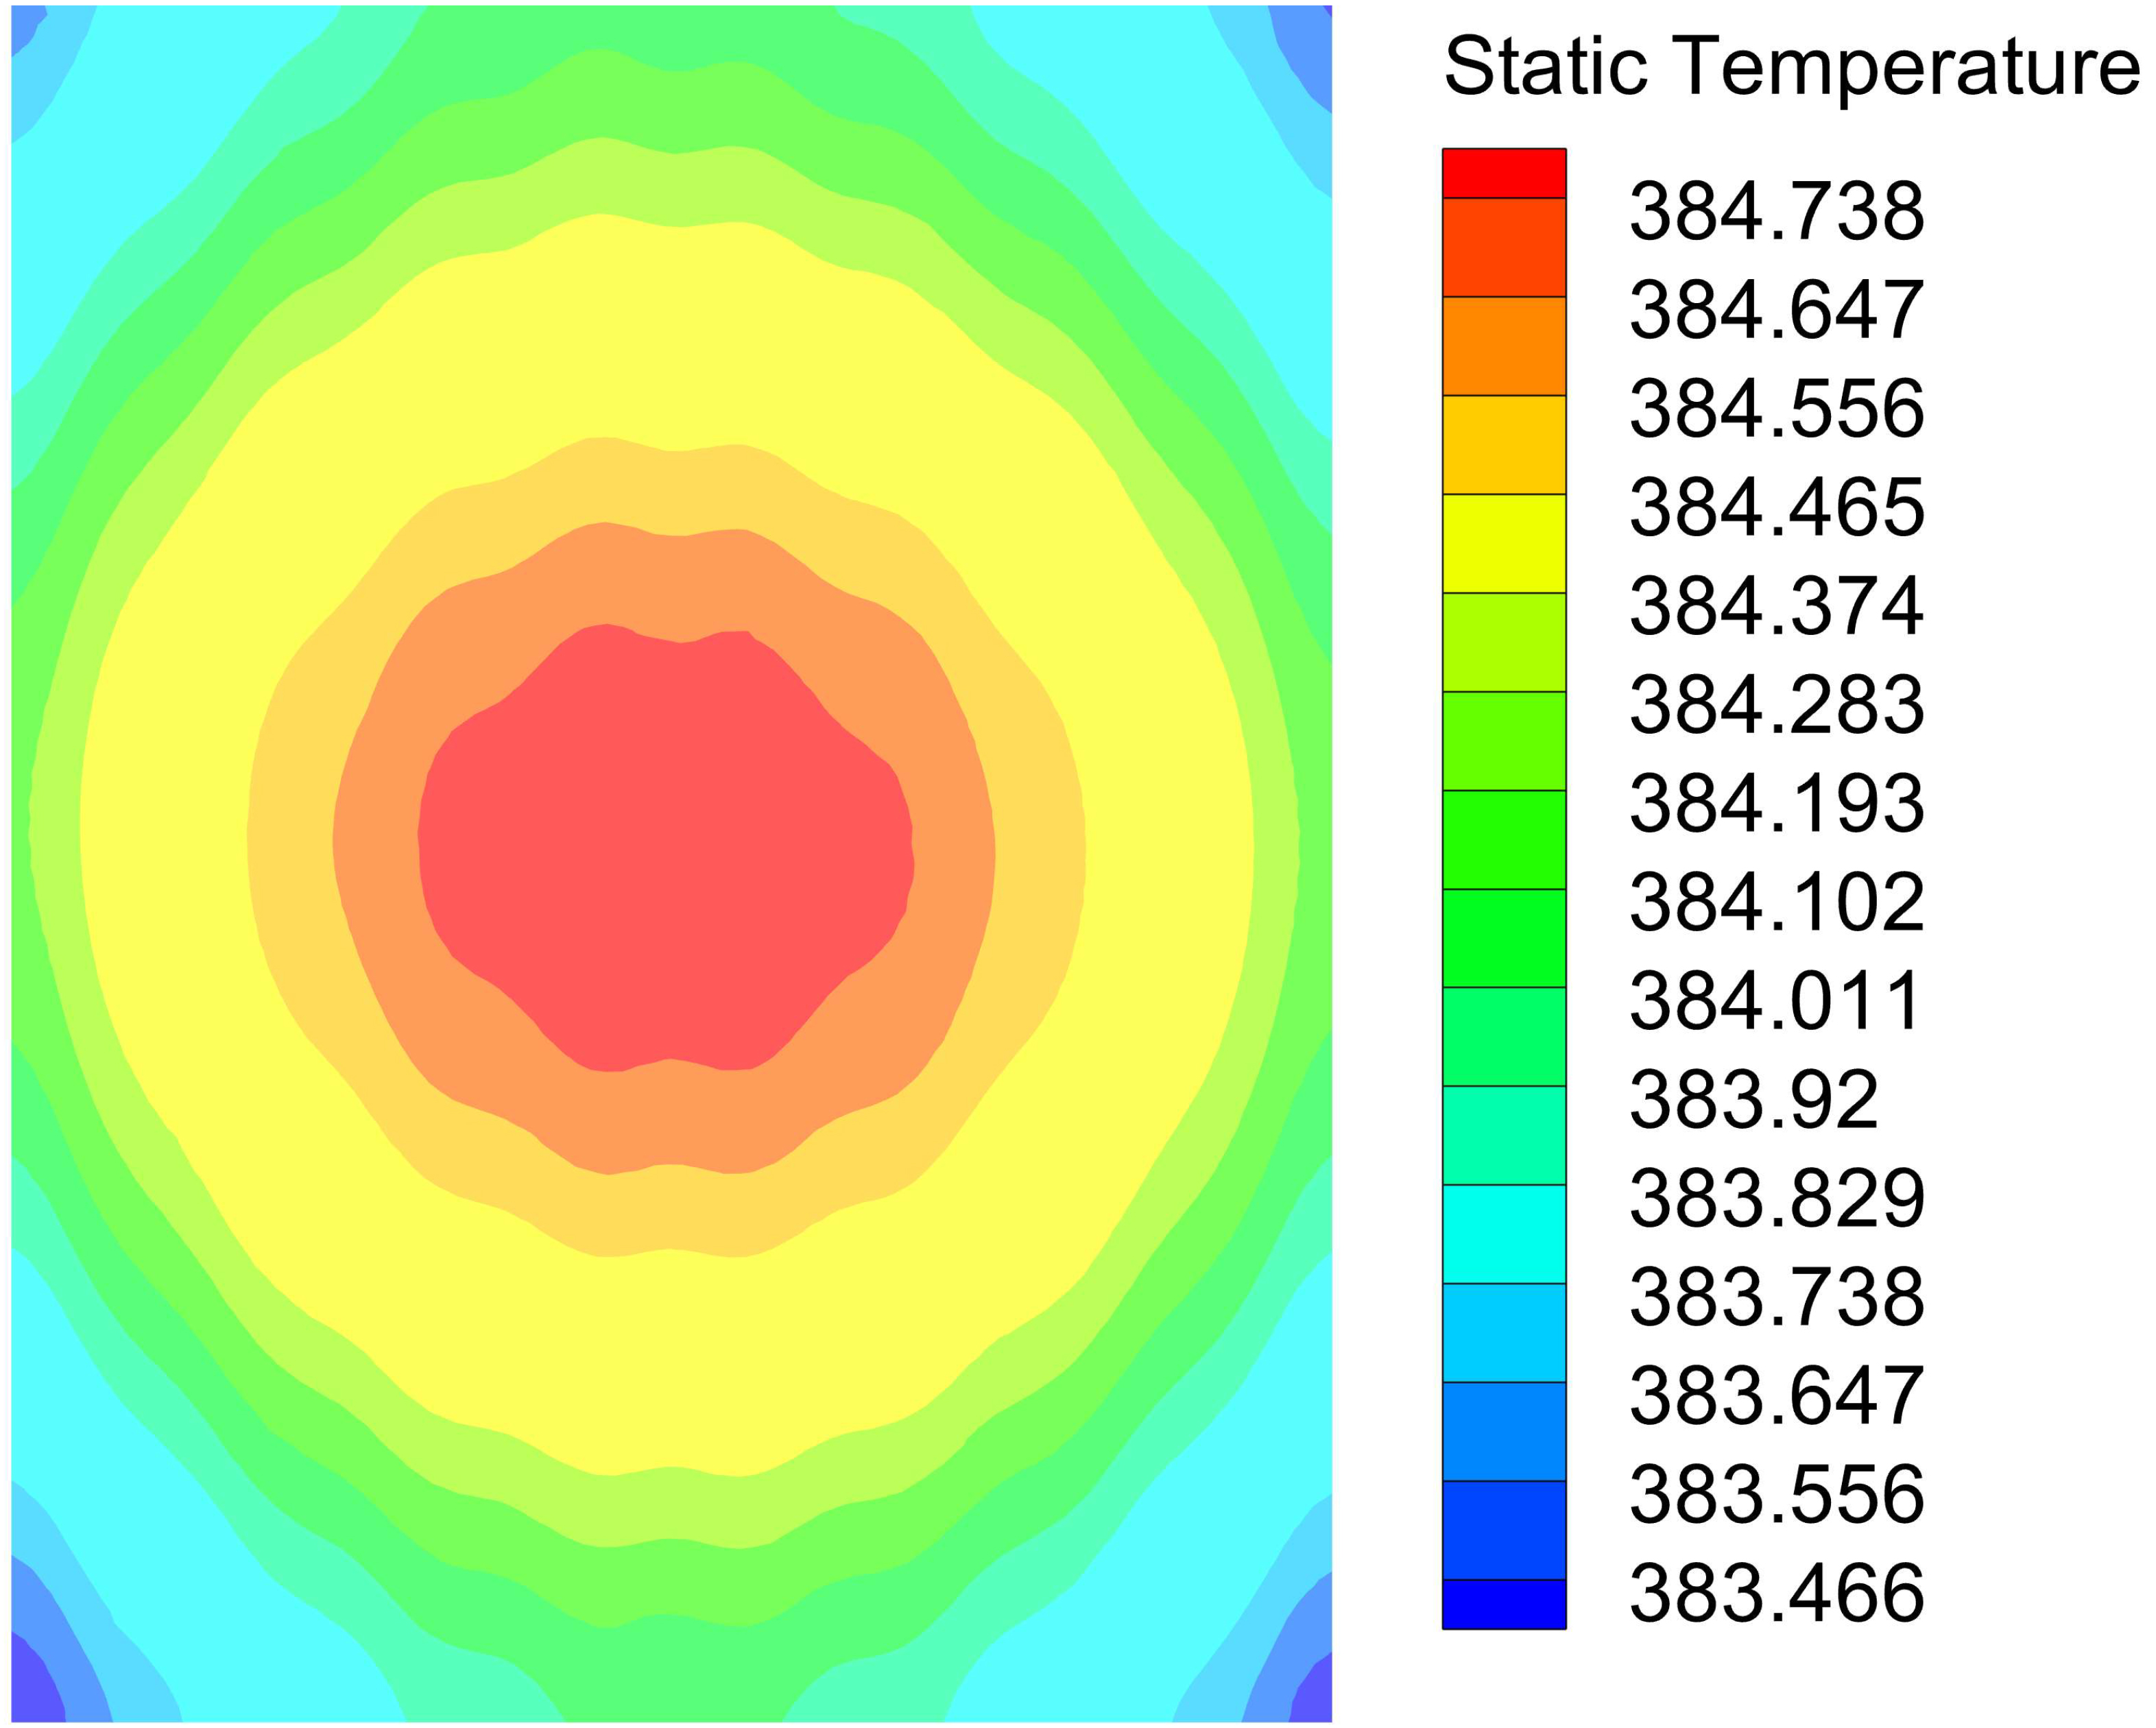
\includegraphics[scale=0.7,width=5cm]{figure14-no.jpg}
		%  \end{minipage}
		}
		   \subfigure[]
		   {
			% \begin{minipage}{5cm}
			 \centering
			 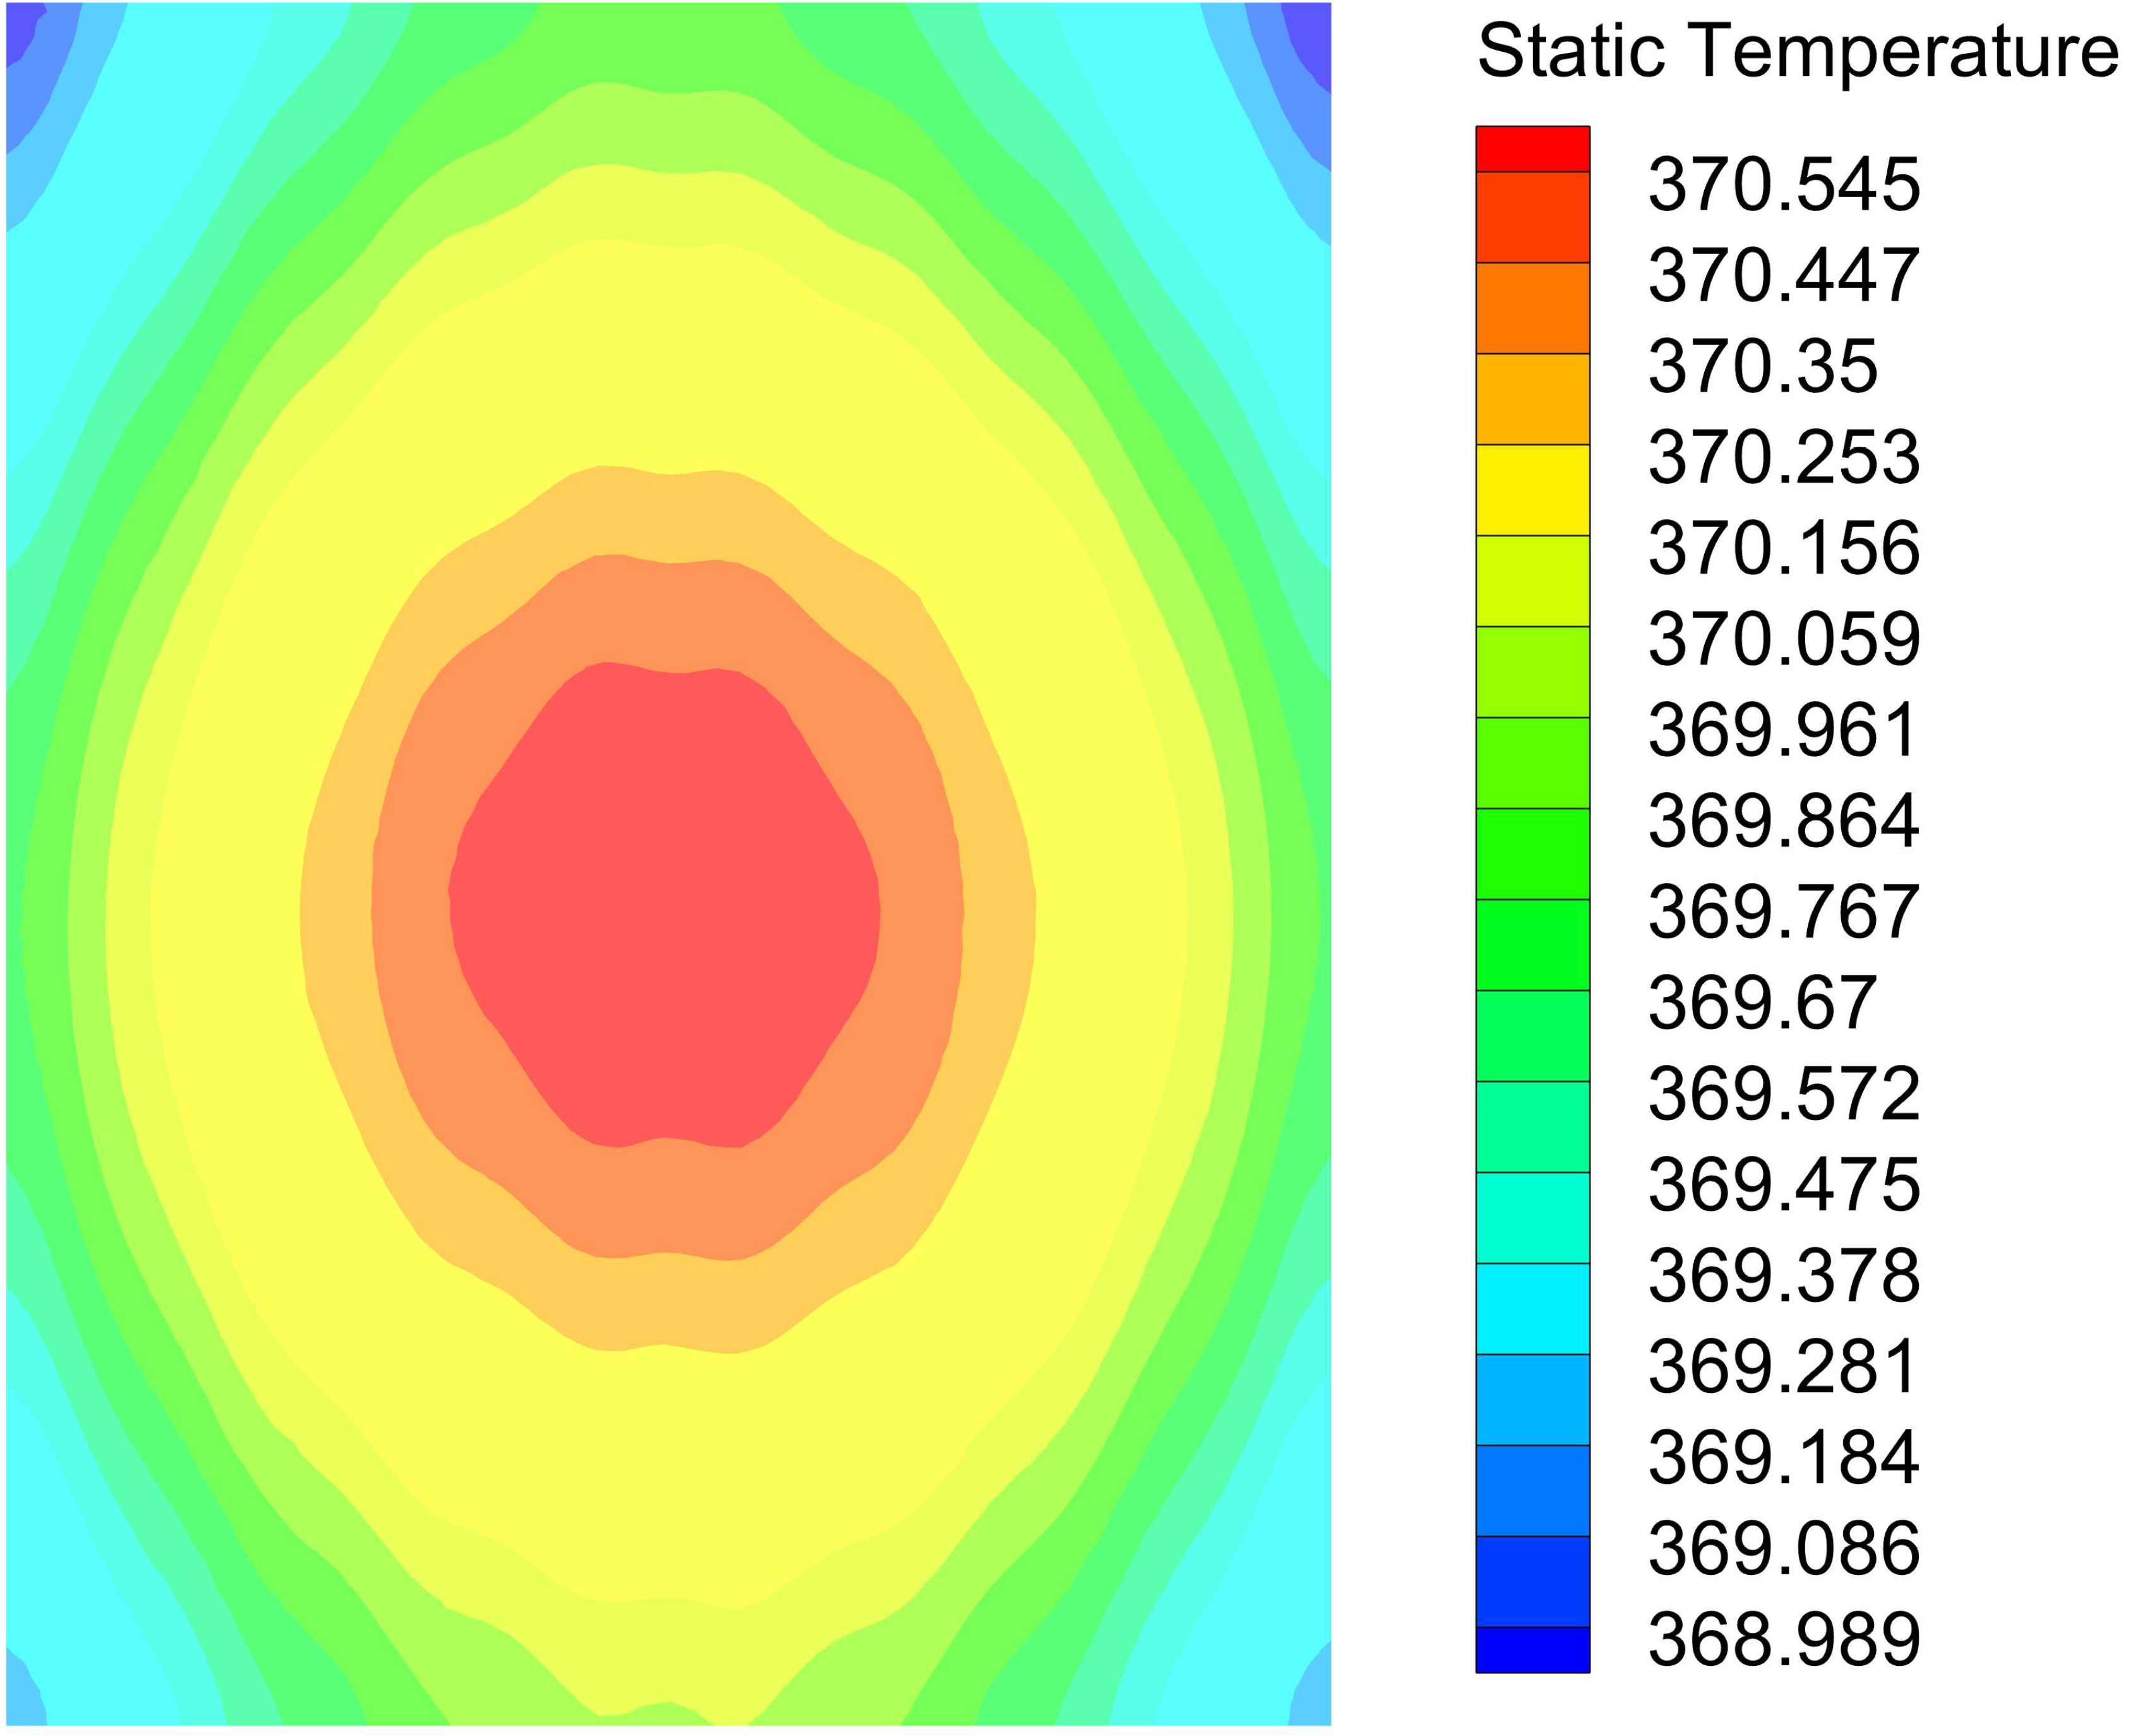
\includegraphics[scale=0.7,width=5cm]{figure14-0.jpg}
			% \end{minipage}
		   }
	   \caption{应用S2S辐射模型前(a)后(b)电子元件表面温度分布}

	   \end{figure}
\end{frame}
\end{document}
%%% TeX代码结束
